% Options for packages loaded elsewhere
\PassOptionsToPackage{unicode}{hyperref}
\PassOptionsToPackage{hyphens}{url}
\PassOptionsToPackage{dvipsnames,svgnames,x11names}{xcolor}
%
\documentclass[
  11pt,
]{article}
\usepackage{amsmath,amssymb}
\usepackage{iftex}
\ifPDFTeX
  \usepackage[T1]{fontenc}
  \usepackage[utf8]{inputenc}
  \usepackage{textcomp} % provide euro and other symbols
\else % if luatex or xetex
  \usepackage{unicode-math} % this also loads fontspec
  \defaultfontfeatures{Scale=MatchLowercase}
  \defaultfontfeatures[\rmfamily]{Ligatures=TeX,Scale=1}
\fi
\usepackage{lmodern}
\ifPDFTeX\else
  % xetex/luatex font selection
\fi
% Use upquote if available, for straight quotes in verbatim environments
\IfFileExists{upquote.sty}{\usepackage{upquote}}{}
\IfFileExists{microtype.sty}{% use microtype if available
  \usepackage[]{microtype}
  \UseMicrotypeSet[protrusion]{basicmath} % disable protrusion for tt fonts
}{}
\usepackage{xcolor}
\usepackage[margin=1in]{geometry}
\usepackage{longtable,booktabs,array}
\usepackage{calc} % for calculating minipage widths
% Correct order of tables after \paragraph or \subparagraph
\usepackage{etoolbox}
\makeatletter
\patchcmd\longtable{\par}{\if@noskipsec\mbox{}\fi\par}{}{}
\makeatother
% Allow footnotes in longtable head/foot
\IfFileExists{footnotehyper.sty}{\usepackage{footnotehyper}}{\usepackage{footnote}}
\makesavenoteenv{longtable}
\usepackage{graphicx}
\makeatletter
\def\maxwidth{\ifdim\Gin@nat@width>\linewidth\linewidth\else\Gin@nat@width\fi}
\def\maxheight{\ifdim\Gin@nat@height>\textheight\textheight\else\Gin@nat@height\fi}
\makeatother
% Scale images if necessary, so that they will not overflow the page
% margins by default, and it is still possible to overwrite the defaults
% using explicit options in \includegraphics[width, height, ...]{}
\setkeys{Gin}{width=\maxwidth,height=\maxheight,keepaspectratio}
% Set default figure placement to htbp
\makeatletter
\def\fps@figure{htbp}
\makeatother
\setlength{\emergencystretch}{3em} % prevent overfull lines
\providecommand{\tightlist}{%
  \setlength{\itemsep}{0pt}\setlength{\parskip}{0pt}}
\setcounter{secnumdepth}{5}
% definitions for citeproc citations
\NewDocumentCommand\citeproctext{}{}
\NewDocumentCommand\citeproc{mm}{%
  \begingroup\def\citeproctext{#2}\cite{#1}\endgroup}
\makeatletter
 % allow citations to break across lines
 \let\@cite@ofmt\@firstofone
 % avoid brackets around text for \cite:
 \def\@biblabel#1{}
 \def\@cite#1#2{{#1\if@tempswa , #2\fi}}
\makeatother
\newlength{\cslhangindent}
\setlength{\cslhangindent}{1.5em}
\newlength{\csllabelwidth}
\setlength{\csllabelwidth}{3em}
\newenvironment{CSLReferences}[2] % #1 hanging-indent, #2 entry-spacing
 {\begin{list}{}{%
  \setlength{\itemindent}{0pt}
  \setlength{\leftmargin}{0pt}
  \setlength{\parsep}{0pt}
  % turn on hanging indent if param 1 is 1
  \ifodd #1
   \setlength{\leftmargin}{\cslhangindent}
   \setlength{\itemindent}{-1\cslhangindent}
  \fi
  % set entry spacing
  \setlength{\itemsep}{#2\baselineskip}}}
 {\end{list}}
\usepackage{calc}
\newcommand{\CSLBlock}[1]{\hfill\break\parbox[t]{\linewidth}{\strut\ignorespaces#1\strut}}
\newcommand{\CSLLeftMargin}[1]{\parbox[t]{\csllabelwidth}{\strut#1\strut}}
\newcommand{\CSLRightInline}[1]{\parbox[t]{\linewidth - \csllabelwidth}{\strut#1\strut}}
\newcommand{\CSLIndent}[1]{\hspace{\cslhangindent}#1}
\usepackage{longtable}
\LTcapwidth=.95\textwidth
\linespread{1.05}
\usepackage{hyperref}
\usepackage{booktabs}
\usepackage{longtable}
\usepackage{array}
\usepackage{multirow}
\usepackage{wrapfig}
\usepackage{float}
\usepackage{colortbl}
\usepackage{pdflscape}
\usepackage{tabu}
\usepackage{threeparttable}
\usepackage{threeparttablex}
\usepackage[normalem]{ulem}
\usepackage{makecell}
\usepackage{xcolor}
\ifLuaTeX
  \usepackage{selnolig}  % disable illegal ligatures
\fi
\usepackage{bookmark}
\IfFileExists{xurl.sty}{\usepackage{xurl}}{} % add URL line breaks if available
\urlstyle{same}
\hypersetup{
  pdftitle={The Czech Constitutional Court Database},
  pdfauthor={Štěpán Paulík, Humboldt Universität zu Berlin, Institut für Sozialwissenschaften},
  colorlinks=true,
  linkcolor={blue},
  filecolor={Maroon},
  citecolor={Blue},
  urlcolor={Blue},
  pdfcreator={LaTeX via pandoc}}

\title{The Czech Constitutional Court Database\thanks{The database itself is available at a \href{https://zenodo.org/records/11618008}{Zenodo Repository} and replication files are available on the author's \href{https://github.com/stepanpaulik/ccc_dataset}{Github account} as well as the \href{https://dataverse.harvard.edu/dataset.xhtml?persistentId=doi\%3A10.7910\%2FDVN\%2FZO0OOG}{JLC Dataverse}.}}
\author{Štěpán Paulík, Humboldt Universität zu Berlin, Institut für Sozialwissenschaften\footnote{\href{mailto:stepan.paulik.1@hu-berlin.de}{\nolinkurl{stepan.paulik.1@hu-berlin.de}}}}
\date{}

\begin{document}
\maketitle
\begin{abstract}
The article at hand introduces a comprehensive foundational database on the Czech Constitutional Court spanning from its inception in 1993 to 2023. The database includes metadata on all decisions, full text corpus, and additional background data on judges and law clerks, filling a gap in high-quality datasets for empirical legal research in the Central and Eastern European region. As one of the first comprehensive court databases in the CEE region, it has the potential to catalyze similar research efforts and contribute to methodologically rigorous empirical legal research in a region of increasing European significance.
\end{abstract}

\section{Introduction}\label{introduction}

It has been traditionally espoused that there has been a divide between the empirically oriented US legal scholarship, stemming from a different perception of the role of courts and judges, and between the rest of the world (\citeproc{ref-hamannGermanFederalCourts2019}{Hamann 2019, 416}). The empirical legal scholarship is occupied with researching whether and to what extent they behave as for example political or strategic actors.(\citeproc{ref-carrubbaWhoControlsContent2012}{Carrubba et al. 2012}; \citeproc{ref-clarkLocatingSupremeCourt2010}{Clark and Lauderdale 2010}; \citeproc{ref-epsteinChoicesJusticesMake1997}{Epstein and Knight 1997}, \citeproc{ref-epsteinStrategicRevolutionJudicial2000}{2000}; \citeproc{ref-lauderdaleScalingPoliticallyMeaningful2014}{Lauderdale and Clark 2014}; \citeproc{ref-sunsteinAreJudgesPolitical2006}{Sunstein et al. 2006}; \citeproc{ref-cameronChapterWhatJudges2017}{Cameron and Kornhauser 2017}; \citeproc{ref-clarkEstimatingEffectLeisure2018}{Clark, Engst, and Staton 2018}; \citeproc{ref-epsteinWhyWhenJudges2011}{Epstein, Landes, and Posner 2011}; \citeproc{ref-kornhauserModelingCollegialCourts1992}{Kornhauser 1992a}, \citeproc{ref-kornhauserModelingCollegialCourts1992a}{1992b}; \citeproc{ref-posnerWhatJudgesJustices1993}{Posner 1993}, \citeproc{ref-posnerHowJudgesThink2010}{2010}; \citeproc{ref-rousseyOverburdenedJudges2018}{Roussey and Soubeyran 2018}).

In contrast to that, judges have been perceived as ``proclaimers of law'' and the law handed down by them, especially in European legal systems such as the one at hand - Czechia. Hamann (\citeproc{ref-hamannGermanFederalCourts2019}{2019}), p.~417 even claims that such a view had hindered robust empirical legal research in Europe. The lack of empirical legal research can be partially blamed on lack of high quality data, a prerequisite for any quantitative empirical research. At least so the story goes until recently. The interest in empirical legal studies has picked up in the last years across the whole continent, including studies on plethora of topics in Germany (\citeproc{ref-arnoldScalingCourtDecisions2023}{Arnold, Engst, and Gschwend 2023}; \citeproc{ref-coupetteQuantitativeRechtswissenschaft2018}{Coupette and Fleckner 2018}; \citeproc{ref-engstEinflussParteinaheAuf2017}{Benjamin G. Engst et al. 2017}; \citeproc{ref-wittigOccurrenceSeparateOpinions2016}{Wittig 2016}), Spain and Portugal (\citeproc{ref-hanrettyDissentIberiaIdeal2012}{Hanretty 2012}), the UK (\citeproc{ref-hanrettyCourtSpecialistsJudicial2020}{Hanretty 2020}) or on the EU institutions (\citeproc{ref-bielenBacklogsLitigationRates2018}{Bielen et al. 2018}; \citeproc{ref-brekkeThatOrderHow2023}{Brekke, Naurin, et al. 2023}; \citeproc{ref-fjelstulHowChamberSystem2023}{Fjelstul 2023}, \citeproc{ref-fjelstulEvolutionEuropeanUnion2019}{2019}; \citeproc{ref-fjelstulTimelyAdministrationJustice2022}{Fjelstul, Gabel, and Carrubba 2022}).

Publications of new high quality publicly accessible data have gone hand in hand with these developments. To the many released comprehensive datasets and databases in the recent years belong namely the Iuropa project's CJEU database (\citeproc{ref-brekkeCJEUDatabasePlatform2023}{Brekke, Fjelstul, et al. 2023}), the German Federal courts (\citeproc{ref-hamannGermanFederalCourts2019}{Hamann 2019}) as well as the German Federal Constitutional Court (\citeproc{ref-engstConstitutionalCourtDatabaseForthcoming}{Benjamin G. Engst, Hönnige, and Gschwend Forthcoming}) databases (for an overview see \citeproc{ref-engstObservationalDatabases2024}{Benjamin G. Engst and Gschwend 2024}). The mushrooming research proves that there is demand for quality data in Europe as well.

To build on and to continue in these efforts, the article at hand presents a Czech Constitutional Court (``CCC'') database, a comprehensive high-quality multi-user database on the CCC. The CCC database is foundational in that it encompasses plethora of data, on which other researches can base their research efforts on, it possesses the capacity to address various research questions, and it adheres to the tidy data principles. The database includes all decisions of the CCC starting from its foundation in 1993 until the end of 2023. Plenty of metadata is included, such as information on the judge rapporteur, subject matter, or concerned legal acts, a complete text corpus, as well additional background information on judges and clerks.

To the best of my knowledge, the CCC database is one of the first, if not the first, comprehensive databases coming out of the Central and Eastern European (``CEE'') region. The CEE region has gotten to the spotlight of the European legal research, among others as a result of various rule of law crises, in which the regional constitutional courts and their interplay with the CJEU have played an important role (\citeproc{ref-kelemenEuropeanUnionAuthoritarian2020}{R. Daniel Kelemen 2020}; \citeproc{ref-kelemenUsesAbusesConstitutional2019}{R. Daniel Kelemen and Pech 2019}; \citeproc{ref-sadurskiPolandConstitutionalBreakdown2019}{Sadurski 2019} and many other articles). Despite that the CEE scholarship has so far produced very little in terms of methodologically rigorous empirical legal research output concerning the role of the judiciary, constitutional courts or judicial politics. The lack of high-quality data is undoubtedly a piece of this puzzle.

To zero in on Czechia, there have been solitary attempts go gather data in some shape or form in the CCC context (\citeproc{ref-harastaAnnotatedCorpusCzech2018}{Harašta et al. 2018}; \citeproc{ref-novotnaCzechCourtDecisions2019}{Novotná and Harašta 2019}), mainly thanks to the Institute of Law and Technology based in Brno, as well as isolated attempts to conduct network analysis or research employing natural language processing and alike methods (\citeproc{ref-chmelZpravodajoveSenatyVliv2017}{Chmel 2017}; \citeproc{ref-eliasekAutomatickaKlasifikaceVyznamovych2020}{Eliášek, Kól, and Švaňa 2020}; \citeproc{ref-harastaCitacniAnalyzaJudikatury2021}{Harašta et al. 2021}; \citeproc{ref-vartazaryanSitOvaAnalyza2022}{Vartazaryan 2022}). Unfortunately, the former group did not always adhere to the principles of high-quality infrastructure, namely the principle of foundationality, espoused by Weinshall and Epstein (\citeproc{ref-weinshallDevelopingHighQualityData2020}{2020}), p.~424, the latter group did not publish data/code at all. Therefore, the effort to put together and to publish a high-quality database on the CCC is more than warranted, especially to enable robust empirical legal scholarship to flourish in the CEE region.

The presented database can serve as an foundation for wide variety of research inquiries, which I will now briefly discuss and in which I delve deeper the \hyperref[capacity]{section 4.1}. Among others, the judicial politics of the CCC may be studied (\citeproc{ref-laxNewJudicialPolitics2011}{Lax 2011}; \citeproc{ref-laxBargainingOpinionAssignment2007}{Lax and Cameron 2007}). The research on dissenting behavior and disagreement on the bench is of particular interested as the studies of Epstein, Landes, and Posner (\citeproc{ref-epsteinWhyWhenJudges2011}{2011}) and Wittig (\citeproc{ref-wittigOccurrenceSeparateOpinions2016}{2016}) could be replicated with the data at hand. The inclusion of decisions of texts as well as references to other decisions enables the point-estimation of court decisions (\citeproc{ref-clarkLocatingSupremeCourt2010}{Clark and Lauderdale 2010}; \citeproc{ref-gschwendAreJudgesPolitical2016}{Gschwend, Sternberg, and Zittlau 2016}). That in combination with the internal chamber structure of the CCC opens the possibility of an inquiry of how consistent is and under what conditions does the consistency of the CCC caselaw vary across its chambers, following up on the theoretical Fjelstul (\citeproc{ref-fjelstulHowChamberSystem2023}{2023}) study on the caselaw consistency across CJEU chambers. The database enables research on the background of justices, such as the role of gender (\citeproc{ref-boydUntanglingCausalEffects2010}{Boyd, Epstein, and Martin 2010}; \citeproc{ref-epsteinHowSocialIdentity2022}{Epstein and Knight 2022}), their education, or their clerk team selection (\citeproc{ref-kromphardtUSSupremeCourt2015}{Kromphardt 2015}; \citeproc{ref-badasGenderAmbitionPotential2023}{Badas and Stauffer 2023}). The last potential usage of the CCC database that immediately springs into mind is the application of various natural language processing methods. For example, one could replicate the research on vagueness of language of the CCC (\citeproc{ref-sternbergNoPublicNo2019}{Sternberg 2019}) or measure the readibility of the CCC decisions (\citeproc{ref-crossleyMovingClassicReadability2019}{Crossley, Skalicky, and Dascalu 2019}; \citeproc{ref-fixEffectOpinionReadability2020}{Fix and Fairbanks 2020}) and link those measures to interesting research question. For example, do the better readable CCC decisions get cited by the CCC more than the less readable (\citeproc{ref-fixEffectOpinionReadability2020}{Fix and Fairbanks 2020}; \citeproc{ref-crossleyMovingClassicReadability2019}{Crossley, Skalicky, and Dascalu 2019})? Does the CCC use vague language in certain areas/for certain reasons more than for others (\citeproc{ref-sternbergNoPublicNo2019}{Sternberg 2019})?

There are a couple of elements that I believe make the CCC to be especially worthy of study. First, the CCC has been vested with large amount of competences: it may review and quash laws in abstract as well as in concrete proceedings initiated by an individual complaint. On top of that, the CCC has broadened its power and may now review even constitutional amendments and historically has not been afraid to step in into politically salient cases.\footnote{In the \emph{Melčák} case, the CCC entered a heated political battlefield by annulling a constitutional amendment, which shortened the term of the Chamber of Deputies, and sparking a drawn out constitutional crisis. The English version of the decision is available at: \url{https://www.usoud.cz/en/decisions/2009-09-10-pl-us-27-09-constitutional-act-on-shortening-the-term-of-office-of-the-chamber-of-deputies}.} Secondly, there is plenty of variance that can give rise to potential research and that is comparable with other constitutional courts: the CCC is internally composed of chambers of differing size and since 2016 the justices rotate between them, justices are allowed to attach separate opinions, or there is a clear role of the judge rapporteur and the court functionaries. That enables and allows to follow up on and build upon the previously mentioned research of impact of chamber system, judicial politics within the chambers (the role of chamber president, judge rapporteur on the opinion (\citeproc{ref-carrubbaWhoControlsContent2012}{Carrubba et al. 2012})), research on judicial efficiency (\citeproc{ref-brekkeThatOrderHow2023}{Brekke, Naurin, et al. 2023}; \citeproc{ref-fjelstulHowCanEU2023}{Fjelstul and Gabel 2023}), or research on judicial decision-making (such as the dissenting behavior). Lastly, the CCC has involved itself in the European space, including the \emph{Landtova case}, in which the CCC pronounced an EU act as \emph{ultra vires} (\citeproc{ref-komarekCzechConstitutionalCourt2012}{Komárek 2012}). Therefore, the database unlocks the potential to empirically research the role of the CCC in and degree of its europeanization within the EU context (\citeproc{ref-jarembaEuropeanizationNationalJudiciaries2019}{Jaremba and Mayoral 2019}).

The main drawback of the CCC institutional setup is the inability to measure the role of political preferences of justices due to the lack of information on justices' votes (\citeproc{ref-martinDynamicIdealPoint2002}{Martin and Quinn 2002}; \citeproc{ref-hanrettyDissentIberiaIdeal2012}{Hanretty 2012}) and the lack of variance in the nomination process.\footnote{As explained bellow, practically all justices of one term have been nominated and appointed by the same President and Senate.} The question indeed remains to what extent is this strand of research relevant for the European context due to the extent of politicization of the nomination process as well as the judicial decision-making being lower than in the US context. Moreover, the database at hand presents observational data of historically a very rigid institution. Therefore, it is difficult but not impossible to devise a quasi-experimental research design.

To name the last contribution of the presented article, the database offers a blueprint for future efforts to build akin databases. In building the database, I attempted to name the variables and to structure the data in a transparent, replicable and comparable way so that any efforts from different courts can mimic my approach without steep costs and efforts.

The article proceeds as follow. In the \hyperref[primer]{section 2}, I introduce the CCC, namely its compositions, its internal organization and its powers to give the reader a little bit of context. In the \hyperref[database]{section 3}, I introduce the CCC database. Therein, I briefly discuss its structure, its creation, and describe its variables. The \hyperref[principles]{section 4} then discusses the adherence of the CCC database to four principles of a high-quality dataset, including its relevance for research, as well as to the adherence of the tidy data principles. The last \hyperref[conclusion]{section 5} concludes.

\section{A Brief Primer on the CCC}\label{primer}

The CCC consists of fifteen justices\footnote{I will proceed with calling the CCC judges as ``justices'' in the SCOTUS fashion (\citeproc{ref-boatrightHistoryMeaningUse2018}{Boatright 2018}) as the CCC is the highest court with constitutional review
  powers.}, out of which one is the president of the CCC, two are vice presidents and twelve associate justices (following the terminology of \citeproc{ref-kosarConstitutionalCourtCzechia2020}{Kosař and Vyhnánek 2020}). These fifteen justices are appointed by the president of the Czech republic upon approval of the Senate, the upper chamber of the Czech two-chamber Parliament. The justices enjoy 10 years terms with the possibility of re-election; there is no limit on the times a justice can be re-elected. The three CCC functionaries are unilaterally appointed by the Czech president.

The appointment procedure is similar to how the SCOTUS justices are appointed as the procedure lays in the hands of the president of the republic and the upper chamber. The minimal requirement for a CCC nominee are 40 years of age, a clean criminal record, a finished legal education and experience in the legal field. Other than that, the nomination is left to the consideration of the President of the Republic. After a nomination, the nominee is firstly interviewed in the constitutional law committee of the Senate, which produces an unbinding recommendation for the plenary Senate hearing. The final binding decision is then made by simple majority of the Senate plenary hearing. This procedure has lead to a situation, in which there is very little variance as to the nominating background of the justices. First, there is no nominating political party akin to the US context or the Spanish context (\citeproc{ref-hanrettyDissentIberiaIdeal2012}{Hanretty 2012}). Second, because the court was established in 1993 and filled within roughly a year of its establishment and because the term of the Czech president is 5 years and all the 3 Presidents, who'd finished their term at the time of writing this article, have been elected twice (for ten years it total), each president has had the chance to appoint all the fifteen members of ``their'' CCC. Therefore, the first term of the CCC has been termed the Václav Havel, the second the Václav Klaus and the third Miloš Zeman terms of the CCC.

Regarding the competences, the CCC is a typical Kelsenian court inspired mainly by the German Federal Constitutional Court. The CCC enjoys the power of abstract constitutional review, including constitutional amendments. The abstract review procedure is initiated by political actors (for example MPs) and usually concerns political issues. Moreover, an ordinary court can initiate a concrete review procedure, if that court reaches the conclusion that a legal norm upon which its decision depends is not compatible with the constitution. Individuals can also lodge constitutional complaints before the CCC. Lastly, the CCC can also resolve separation-of-powers disputes, it can \emph{ex ante} review international treaties, decide on impeachment of the president of the republic, and it has additional ancillary powers (for a complete overview, see \citeproc{ref-kosarConstitutionalCourtCzechia2020}{Kosař and Vyhnánek 2020}).

The CCC is an example of a collegial court. From the perspective of the inner, the CCC can decide in four bodies: (1) individual justices in the role of judge rapporteur, (2) 3-member chambers (\emph{senáty}), (3) the plenum (\emph{plénum}), and (4) special disciplinary chamber. The 3-member chambers and the plenum play a crucial role. The plenum is composed of all justices, whereas the four 3-member chambers are composed of the associate justices. Neither the president of the CCC or her vice-presidents are permanents members of the 3-member chambers. Until 2016, the composition of the chambers was static. However, in 2016, a system of regular 2-yearly rotations was introduced, wherein the president of the chamber rotates to a different every 2 years. I am of the view that such a institutional change opens up potential for quasi-experimental research similar to the Gschwend, Sternberg, and Zittlau (\citeproc{ref-gschwendAreJudgesPolitical2016}{2016}) study utilizing judge absences within the 3-member chambers of the German federal constitutional court. In general, the plenum is responsible for the abstract review, whereas the 3-member chambers are responsible for the individual constitutional complaints.

In the chamber proceedings, decisions on admissibility must be unanimous, whereas decisions on merits need not be, therefore, a simple majority of two votes is necessary to pass a decision on merits. In the plenum, the general voting quorum is a simple majority and the plenum is quorate when there are ten justices present. The abstract review is one of the exceptions that sets the quorum higher, more specifically to 9 votes.

A judge rapporteur plays a crucial role (\citeproc{ref-chmelZpravodajoveSenatyVliv2017}{Chmel 2017}; \citeproc{ref-horenovskyProcessMakingConstitutional2015}{Hořeňovský and Chmel 2015} study the large influence of the judge rapporteurs at the CCC). Each case of the CCC gets assigned to a judge rapporteur. The assignment is regulated by a case allocation plan.\footnote{The original term is \emph{rozvrh práce}, which is usually translated as a \emph{work schedule}, however, I borrow the term \emph{case allocation plan} from Hamann (\citeproc{ref-hamannGermanFederalCourts2019}{2019}), p.~673.} They are tasked with drafting the opinion, about which the body then votes. The president of the CCC (in plenary cases) or the president of the chamber (in chamber cases) may re-assign a case to a different judge rapporteur if the draft opinion by the original judge rapporteur did not receive a majority of votes. Unfortunately, the CCC does not keep track of these reassignments.\footnote{More specifically, some decisions mention the reassignment. However, not all do, therefore an attempt to retrieve the information from the texts was highly unreliable. According to my internal insight, the CCC should always pass a short procedural decision when a reassignment takes place. I unsuccessfully attempted to retrieve the information with the right to information as the procedural decision is not available in electronic form and retrieving the full information would thus entail manually going through all paper files.}

The act on the CCC allows for separate opinions. They can take two forms: dissenting or concurring opinions. Each justice has the right to author a separate opinion, which then gets published with the CCC decision. It follows that not every anti-majority vote implies a separate opinion, it is up to the justices to decide whether they want to attach a separate opinion with their vote. Vice-versa, not every separate opinion implies an anti-majority vote, as the justices can attach a concurring opinion. In contrast to dissenting opinion, when a justice attaches a concurring opinion, they voted with the majority but disagree with its argumentation.\footnote{Which makes it difficult to, for example, conduct the same point-estimation with data on dissenting behavior of justices as Hanretty (\citeproc{ref-hanrettyDissentIberiaIdeal2012}{2012}) has done on the Portuguese and Spanish Constitutional Courts.}

The CCC justices can hire their clerk teams. Each justice is required to have at least one clerk. The clerk is appointed by the president of the CCC on the nomination of the said justice. The clerk must have a clean criminal record and a finished legal degree. Other than that there are no requirements on the clerks. The term of the clerks may not exceed the term of the nominating justice. The clerks are usually tasked with drafting decisions and, in narrowly defined cases, can be instructed by the justice to decide on their behalf when an application does not meet even the minimal requirements.

It may be concluded that the CCC takes after the american model of selection of justices, with the president of the republic and the upper chamber being in the spotlight, but is also a typical example of a Kelsenian specialized court with concentrated constitutional review. The CCC stands out in how powerful its constitutional review is, having attracted the power to review even constitutional amendments, thus, the CCC is a powerful player in the Czech political system. While the appointment procedure of the justices may be compared to the SCOTUS, its role within the constitutional system is akin to the European constitutional courts, with the German federal constitutional court at its forefront. Its doctrinal approaches and methods, such as the test of proportionality or test of rationality, have often been adopted by the CCC. Its power to review even constitutional amendments may then be comparable to the Supreme Court of Israel. The internal organization of the CCC gives room for strategic or policy considerations of its justices. Not only due to the similarities with the constitutional adjudication powerhouses but also due to its own idiosyncrasies, I believe the CCC to be a worthy object of empirical legal research as the conclusions drawn from research of the CCC may be after a careful consideration be extended beyond a mere case study on the CCC.

\section{Description of the CCC database}\label{database}

Now that the CCC has been introduced in the previous section, I move on to describing the content and structure of the dataset in this section.

\subsection{Case Inclusion}\label{case-inclusion}

The CCC database includes all publicly available CCC decisions from its foundation until the end of 2023\footnote{The article makes a snapshot of the data up to a certain point in time. However, the data will be updated regularly to enable scholars to research the perhaps most relevant recent trends.}, that is 93826 decisions, as well as background information on its 50 justices and their 221 clerks. All the data was first web scraped from the official CCC website \href{https://nalus.usoud.cz/Search/Search.aspx}{Nalus}. Nalus is an official publicly accessible database in the form of a website, on which the CCC publishes all its decisions on merits and admissibility. Nalus includes all procedural decisions decided after 1.1.2007, procedural decisions before that date may be missing without a specification as to which are missing.\footnote{The manual to the Nalus database says ``All decisions of the Constitutional Court that terminated proceedings from the beginning of the Constitutional Court's activity in 1993 until the end of 2006 (approximately 26,000 decisions) were automatically imported into the NALUS database.''}

The web scraping was followed by intense data cleaning and data wrangling processes. A lot of the information was transformed to a more readily form. In the last step, some information was mined from the texts or other metadata of the decisions (such as composition of the bench). The CCC database is accompanied by a comprehensive codebook, which contains detailed explanation of its structure, parts and all variables contained therein.\footnote{Available at: \url{https://zenodo.org/records/11618008} as well as \url{https://dataverse.harvard.edu/dataset.xhtml?persistentId=doi\%3A10.7910\%2FDVN\%2FZO0OOG}}

\subsection{Structure of the CCC Database}\label{structure-of-the-ccc-database}

The structure of the CCC database can, on a very basic level, be divided into the master decision-level table (\emph{ccc\_metadata}), decision-variable level tables and justice-level/clerk-level tables. The decision-variable level tables are linked to the master table by the decision identifier and the justice/clerk-level tables are connected by the judge identifier and clerk identifier. I now go over each level of the structure. For the clarity of the ensuing description of the database, fig.~\ref{fig:database-diagram} presents a diagram of the schema of the CCC database, which can be used as a reference point. Tab. \ref{tab:skim} contains summary statistics of the whole database.

\begin{figure}
\centering
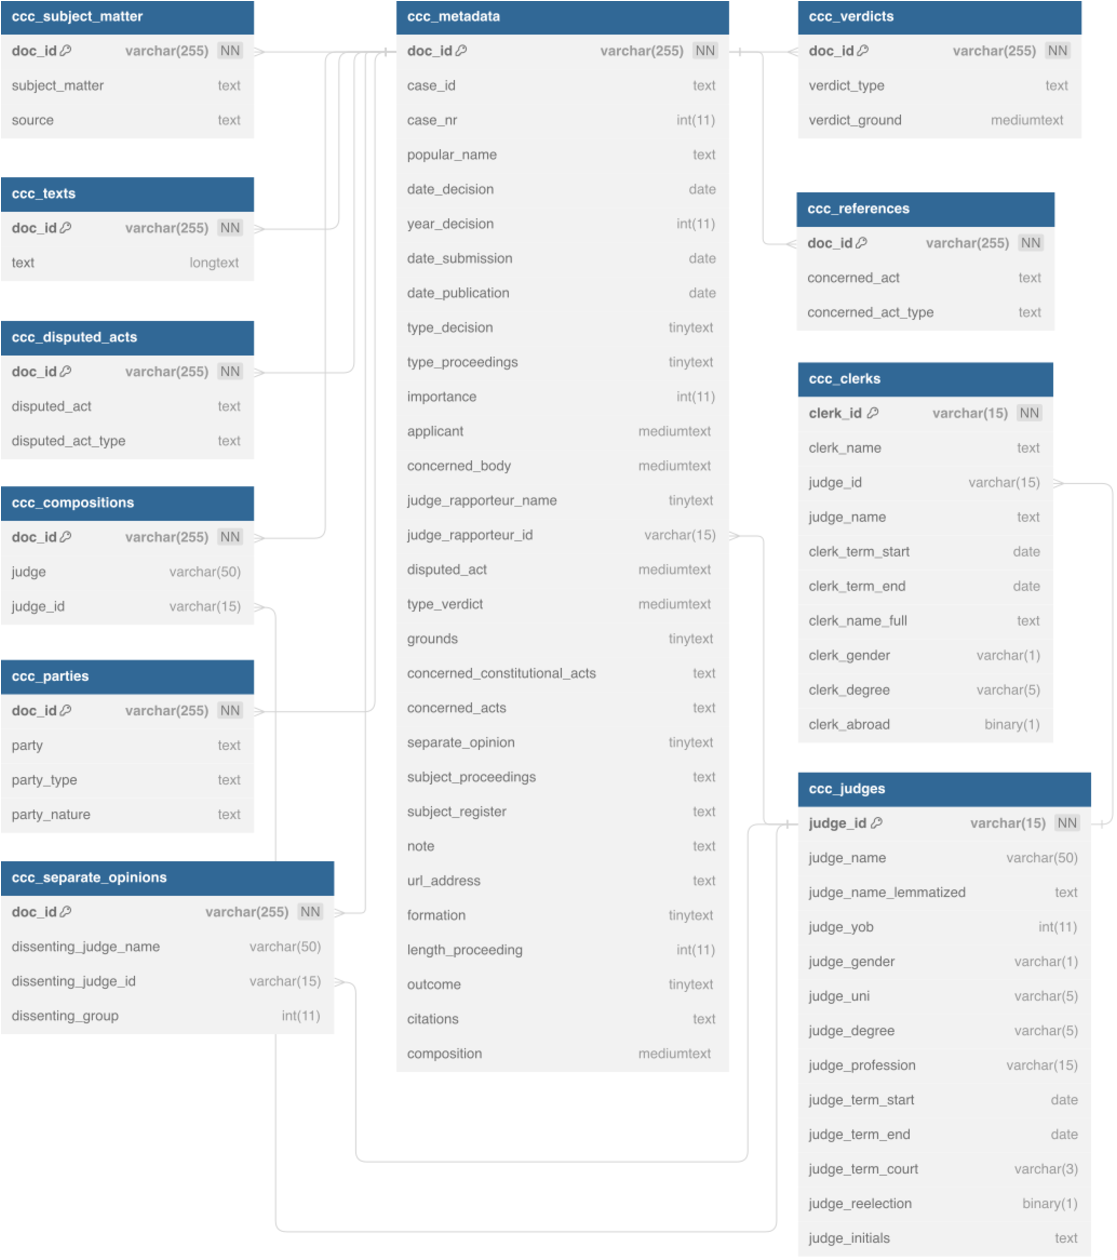
\includegraphics{The_Czech_Constitutional_Court_Database_files/figure-latex/database-diagram-1.pdf}
\caption{\label{fig:database-diagram}A diagram of the CCC database schema. The main master table is the ccc\_metadata table, to which all the decision-variable level tables are linked via the doc\_id unique identifier. The ccc\_judges table is directly connected to the ccc\_metadata via the judge\_rapporteur\_id variable and indirectly linked via the ccc\_composition table.}
\end{figure}

\subsubsection{Master Table}\label{master-table}

The whole database is guided by and revolves around a master \emph{ccc\_metadata} table, as seen on the fig.~\ref{fig:database-diagram}. The master table contains multiple types of information. The general case information variables contain information a unique identifier of the decisions, a non-unique identifier of the case that may include more than one decisions, and the dates at which the application was lodged and the decision decided. Procedural variables concern whether the decision was a \emph{usnesení} or \emph{nález}\footnote{Roughly speaking \emph{nález} is a decision on merits, whereas \emph{usnesení} is a decision on admissibility or a procedural decision.}, what type of procedure the decision was made in, such as abstract review or constitutional complaint procedure, or on what type of grounds the decision was based. Background variables concern among others parties before the CCC, which are identified (a natural person, a legal person, a court etc.), the body whose decision was under review (typically which court), the type of decision being reviewed and alike. Moreover, the data on the subject proceedings (relates to the area of constitutional law) and subject register (the pertaining area of general law such as criminal-proof, civil damages, or administrative proceedings) is included. Such variables are especially useful for controlling for specific features of cases that may have confounding potential. Lastly, miscellaneous variables contain for example an URL address to the decision in the Nalus database or a note, which typically contains a link to the press release.\footnote{The note to press release lends itself to creating a similar measure of case salience as Epstein and Segal (\citeproc{ref-epsteinMeasuringIssueSalience2000}{2000}).}

\begin{table}

\caption{\label{tab:skim}Overview of the tables of the CCC database as well as summary statistics.}
\centering
\begin{tabular}[t]{l|l|r|r}
\hline
Table & Observation Level & \# Observations & \# Variables\\
\hline
ccc\_metadata & decision & 93826 & 30\\
\hline
ccc\_texts & text & 93826 & 2\\
\hline
ccc\_compositions & sitting justice & 219827 & 3\\
\hline
ccc\_references & reference & 543641 & 3\\
\hline
ccc\_metadata & separate opinion & 1154 & 4\\
\hline
ccc\_subject\_matter & subject matter & 351943 & 3\\
\hline
ccc\_parties & party & 237144 & 4\\
\hline
ccc\_verdicts & verdict & 103142 & 3\\
\hline
ccc\_judges & judge & 55 & 14\\
\hline
ccc\_clerks & clerk-judge & 376 & 10\\
\hline
\end{tabular}
\end{table}

\subsubsection{Decision-variable-level Tables}\label{decision-variable-level-tables}

Some of the aforementioned variables may contain more than one observation per decision. In effect, to keep all information in one table would entail breaking the tidy data principle that each row contains one observation as the observation in the \emph{ccc\_table} is one decision. To resolve this issue, some variables of the master table are stored as a nested list and then unnested into separate tables, in which the observation is a decision-variable level.\footnote{While the tables themselves are only on the variable level, i.e.~a separate opinion forms the observation of the \emph{ccc\_separate\_opinions} table, I am employing the term decision-variable to refer to the group of tables that are based on the unnested variables from the \emph{ccc\_metadata} table as they simply contain unnested information for each decision.} These tables are connected to the main table by the unique decision identifier. The unnested tables include, to name a few, \emph{ccc\_references} (contains references to CCC caselaw found in the texts of the decisions), \emph{ccc\_subject\_matter} (contains subject matters of a decision), \emph{ccc\_parties} (contains information on the parties, both the applicant and the concerned body, before the CCC), or \emph{ccc\_compositions} (contains the bench composition with a link to the \emph{ccc\_judges} table via the judge identifier).

Lastly, the \emph{ccc\_texts} contains full texts of the decisions, which unlocks plethora of potential research endeavors utilizing quantitative text analysis or various machine learning endeavors. The texts have underwent a very little pre-processing as the texts in the Nalus database are in a good state. Most of the html tags have been removed apart from paragraph tag (mostly in the form of one or more \emph{\textbackslash n} tags). As the decisions have no clear structure, the texts have been kept as a whole\footnote{I have been able to partition the text into an implicit structure such as the heading, procedure history, parties' arguments, or court arguments using a supervised machine learning algorithm. However, the decisions do not lend themselves to a simple and reliable regex partitioning. The only clear general rule is that the first paragraph most of the time contains the heading of the decision, in which the composition as well as the parties of the case can be located.} and any researcher intending to run any NLP task can simply split them up into a unit they deem fit (tokens, sentences, paragraphs etc.). A number of variables have already been mined from these texts. To name two, the compositions of sitting benches have been mined using various regex variations of the justices' names and dissenting opinions as well as their relationships to each other (whether more judges signed one dissenting opinion or whether they dissented separately) have been mined from the texts.

\subsection{Justice-level and Clerk-level Tables}\label{justice-level-and-clerk-level-tables}

Justice-level and clerk-level variables contain information on the individual justices and clerks respectively. The information was collected partly automatically and partly manually from the official profiles of \href{https://www.usoud.cz/soucasni-funkcionari-a-soudci}{current justices}, \href{https://www.usoud.cz/emeritni-funkcionari-a-soudci}{former justices}, and \href{https://www.usoud.cz/asistenti-soudcu}{clerks} at the CCC website, as well as \href{https://cs.wikipedia.org/wiki/Seznam_soudců_Ústavního_soudu_České_republiky}{Wikipedia profile pages of the justices}. The CCC database includes information on the terms of the justices, their age and gender, their alma mater, highest reached degree, as titles play an especially important ``ceremonial'' role in the Czech legal environment, their professional background before they became a judge\footnote{Coded as the last profession before they started their CCC term.}, or information on whether the justice ran for a reelection as the Czech Constitution and the act on the CCC allow for reelection of justices after their 10 year term runs out.

Secondly, the \emph{ccc\_clerks} table includes information on all 221 clerks that have served in the CCC's history. The table on clerks contains information, such as under which judge they served, what was their term, what is their gender, education, or whether they studied abroad. Because one clerk could have over time served under more than one judge, the observation of the table is at the term of the clerk level. Therefore, there are more rows than there are unique clerks. I believe inclusion of such an information on clerks makes the dataset quite unique and opens up a lot of avenues for research.

\section{Principles Guiding the CCC database}\label{principles}

The Czech Constitutional Court database is a ``multi-user dataset'' created in a principled manner. Epstein et al. (\citeproc{ref-epsteinIntroductionEmpiricalLegal2014}{2014}), p.~14 define a multi-user dataset as a dataset created with the purpose of ``{[}r{]}ather than collect data to answer particular research questions {[}\ldots{]} the idea is to amass a dataset so rich in content that multiple users, even those with distinct projects, can draw on it.''

Accordingly, the CCC database upholds the principles of a high-quality datasets espoused by Weinshall and Epstein (\citeproc{ref-weinshallDevelopingHighQualityData2020}{2020}), p.~424, namely that the database is (1) capable of addressing real-world problems, (2) accessible, (3) reproducible and reliable, and (4) foundational.\footnote{I decided to skip the principle of sustainability as I do not see the benefit of discussing it separately, most of its issues are answered in the other sections.} The data structure also follows the principles of tidy data. According to Wickham (\citeproc{ref-wickhamTidyData2014}{2014}), tidy data are data with such a tabular structure, i.e.~data with a column and row structure, that stick to the following principles

\begin{enumerate}
\def\labelenumi{(\arabic{enumi})}
\tightlist
\item
  every column is a variable,
\item
  every row is an observation,
\item
  every cell is a single value.\footnote{This does not necessarily apply to the nested variables in the \emph{ccc\_dataset}. I stil believe though that the nested variable can be viewed as a one value from the decision-level perspective. When unnested, it naturally contains more values on the decision-variable level.}
\end{enumerate}

I now go over and discuss the Weinshall and Epstein (\citeproc{ref-weinshallDevelopingHighQualityData2020}{2020}) principles one by one and describe them in detail.

\subsection{Capacity to Address Real-World Problems}\label{capacity}

In the words of Weinshall and Epstein (\citeproc{ref-weinshallDevelopingHighQualityData2020}{2020}), ``By definition, data infrastructure should promote innovation, inventions, and insights. Although no product can guarantee these ends, infrastructure aimed at solving (or developing implications for) real-world problems increases the odds of success.'' With the database at hand I hope to enable data- and evidence- based research on the CCC. I now present two examples that corroborate the capacity of the CCC database to address real-world problems and research concerns. The disclaimer is that the goal of presenting these simplified examples is not to draw any inference but rather to show the potential of using the dataset ``to develop real-world implications and contribute to public and academic discourse on pressing legal-political issues''. (\citeproc{ref-weinshallDevelopingHighQualityData2020}{Weinshall and Epstein 2020, 427})

\subsubsection{Clerks}\label{clerks}

The first brief example concerns the law clerks. Kosař and Vyhnánek (\citeproc{ref-kosarConstitutionalCourtCzechia2020}{2020}) argue that the clerks at the CCC play an especially vital and underappreciated role: ``The initial idea of the legislature was to grant each Justice one law clerk who would take administrative burdens unrelated to substantive decision-making off the Justices' shoulders. Yet the reality is different. First, due to the growing caseload, the number of law clerks per Justice increased gradually; today, each Justice has three law clerks. Moreover, law clerks de facto prepare drafts of most CCC judgments and decisions, and the real administrative burden has been `outsourced' to secretaries of the cabinets.'' The difficulty of studying the role of clerks was highlighted in the Clark, Engst, and Staton (\citeproc{ref-clarkEstimatingEffectLeisure2018}{2018}) study on the effects of leisure on judicial performance. In the existing studies on clerks, their influence on the final decision as ``an information source'' (\citeproc{ref-kromphardtUSSupremeCourt2015}{Kromphardt 2015}) or the influence of their gender on their career choice to become a clerk have been researched (\citeproc{ref-badasGenderAmbitionPotential2023}{Badas and Stauffer 2023}).

\begin{figure}
\centering
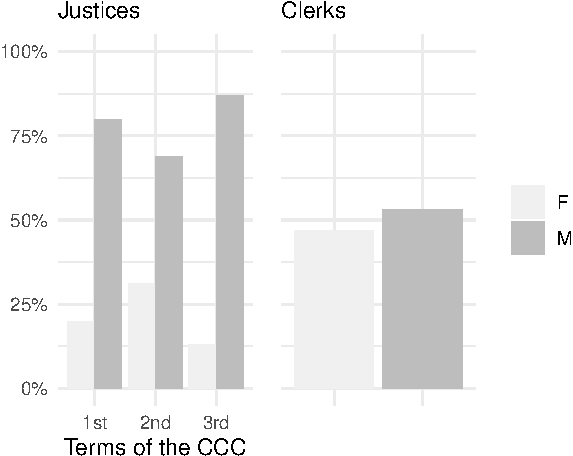
\includegraphics{The_Czech_Constitutional_Court_Database_files/figure-latex/gender-distribution-1.pdf}
\caption{\label{fig:gender-distribution}Comparison of proportions of genders among justices (on the left) and among their clerks (on the right). The X axis of the left bar chart signifies the terms of the CCC, which roughly correspond to decades.}
\end{figure}

Badas and Stauffer (\citeproc{ref-badasGenderAmbitionPotential2023}{2023}) have discovered that women are in general under-represented among law clerks and that one of the reasons behind under-representation of female clerks is that ``female law students may have lower levels of ambition compared to men. (\ldots) Examining potential sources of this difference, we find that while women view themselves to be just as qualified for these positions as men, men are more willing to apply with lower feelings of qualification. Likewise, while women and men report similar levels of encouragement, more encouragement is required before women express ambition to hold these posts.'' In two studies on the gender equality in the Czech judiciary, Havelková (\citeproc{ref-havelkovaGenderEqualityLaw2017}{2017}) and Urbániková, Havelková, and Kosař (\citeproc{ref-urbanikovaArtWaitingHumbly2023}{2023}) have revealed that at first glance the representation of women within the Czech judiciary is rather high. However, structurally, the distribution is vertically unequal: female judges dwell on the first-instance courts and take care of the run-of-the-mill decision-making, whereas male judges are over-represented in the upper echelons of the judiciary, which exert higher influence over doctrinal development, and occupy the judicial functionary positions, which mainly take care of court administration. These studies raise two questions: (1) is the representation of women similarly vertically unequally distributed as that of the justices and (2) is there a discrepancy between the proportion of women among graduates and law clerks?

For the purpose of showing the capability of solving real-world problems, I present concise descriptive statistics in an attempt to answer the question whether there is a discrepancy between the representation of women among clerks, graduates and justices. While the distribution of gender among clerks at the CCC cannot be compared against clerks at lower instance court, as there is no data available, it can at least be compared against the distribution among CCC justices. Tab. \ref{fig:gender-distribution} confirms the gender discrepancy among justices, however, it also reveals that the representation is roughly equal among clerks. It appears then that the unequal vertical distribution may necessarily not be the case among clerks. To answer the second question, I collected data by Eurostat on the gender distribution among law graduates in Czechia between 2015-2021 (\citeproc{ref-eurostatDistributionMaleFemale2024}{Eurostat 2024}) and appended it to the CCC database data.
I compared the proportion of women among thee CCC justices, their clerks and the law graduates.

There are 22 \% of female justices out of the total number of 41 judges, there are 47.3 \% of female clerks out of the total number of 203 clerks, and there are 58.6 \% of female law graduates out of the total number of 1453 law graduates. The discrepancy between clerks and graduates less pronounced but it is still rather pronounced. Women are overrepresented among the law graduates and the overrepresentation does not reflect among clerks. At least the representation remains still roughly equal. As the time goes by, predominatly men reach the higher echelons despite the overrepresentation of women at the starting line. In line with the Badas and Stauffer (\citeproc{ref-badasGenderAmbitionPotential2023}{2023}) paper, one could conduct a similar study in the Czech context and draw policy implications, as to how to resolve the underrepresentation. Lastly, interestingly, Fig. \ref{fig:gender-clerks-judges} reveals that male and female justice seem to have different preferences regarding their clerks. The male CCC justices seem to hire clerks of both genders equally whereas female CCC justices seem to hire more male clerks.

\begin{figure}
\centering
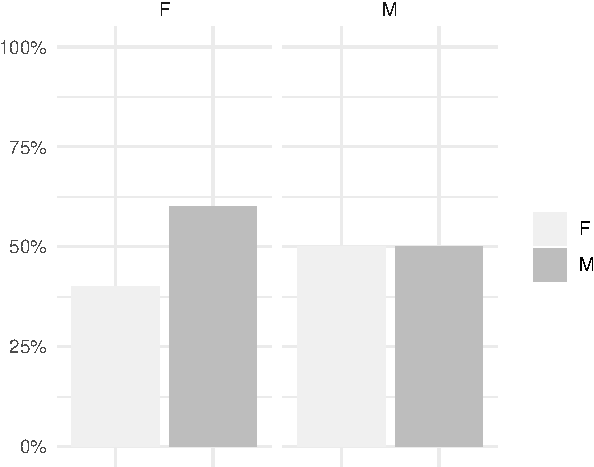
\includegraphics{The_Czech_Constitutional_Court_Database_files/figure-latex/gender-clerks-judges-1.pdf}
\caption{\label{fig:gender-clerks-judges}The gender composition of the clerk teams facetted by the gender of the hiring justice. The gender composition of the clerk teams of female justices is on the left and their male counterparts are on the right.}
\end{figure}

\subsubsection{Dissenting behavior of justices}\label{dissenting-behavior-of-justices}

The second example concerns dissenting behavior of justices. Research on judicial coalitions at the CCC has revealed that the third period of CCC between 2013-2023 is rather polarized and that there are two big coalitions of judges that clash against each other in the plenary proceedings. The division has been coined as left-right or progressive-conservative (\citeproc{ref-chmelCoOvlivnujeUstavni2021}{Chmel 2021}; \citeproc{ref-smekalMimopravniVlivyNa2021}{Smekal et al. 2021}; \citeproc{ref-vartazaryanSitOvaAnalyza2022}{Vartazaryan 2022}). The articles rely primarily on network analysis of the dissenting opinions in the plenary proceedings and make strong conclusions based on a rather superficial descriptive analysis.

To make the previously laid out inference more robust, I predict that should the relationships from the plenum indeed exist, they should also carry over to the 3-member chamber proceedings. In other words, my hypothesis is that chambers composed of judges from both coalitions will be more likely to show disagreement in the form of dissenting opinion. They hypothesis is that 3-member chamber decisions composed of members of both judicial coalitions show higher likelihood of occurance of a dissent. If this shows to be true, it would provide further evidence to the two coalition theory of the CCC (\citeproc{ref-chmelCoOvlivnujeUstavni2021}{Chmel 2021}; \citeproc{ref-vartazaryanSitOvaAnalyza2022}{Vartazaryan 2022}; \citeproc{ref-smekalMimopravniVlivyNa2021}{Smekal et al. 2021}).

\begin{table}
\centering
\caption{\label{tab:coalitions}The total number as well as the percentage of the 3-member chamber decisions containing a separate opinion (SO) depending on whether the composition was made up of justices either from both coalitions (mixed) or from either coalition (full)}
\centering
\begin{tabular}[t]{l|r|r|l}
\hline
Composition & \# with SO & Total & \% with SO\\
\hline
Mixed & 65 & 982 & 6.62\%\\
\hline
Full & 11 & 597 & 1.84\%\\
\hline
\end{tabular}
\end{table}

To test these theoretical expectations, I manually annotated which justices of the 3rd term were from which coalition according to the aforecited literature. Otherwise I built upon the CCC database. The selection of decisions has been narrowed: the admissibility decisions of the 3-member chambers must be made unanimously, concurring decisions therein are a rarity. Therefore, I filtered the decisions in the ccc\_metadata table by the grounds variable to include only decisions on merits. Because the coalition theory applies only to the 3rd term of the CCC roughly between 2013 and 2023, the decisions were further filtered by the year of decision variable. In the end, 1584 3-member chamber decisions on merits have been included in the analysis. For each of these decisions I filtered the 3 justices that decided the case in the ccc\_compositions table using the decision identifier of the 1584 decisions. I then compared those against the vectors of justices' name of either coalition. If the 3 justices all matched against either of the coalitions, I flattened the filtered compositions table into a decision level by imputing the value ``full'', whereas if only 2 justices on the bench were from one coalition and the 3rd justice was from another, I imputed the value ``mixed''. I then joined this filtered table to the filtered metadata table by the decision identifier variable. Lastly, I grouped by the separate opinion table by the decision identifier and then flattened the table to contain only the information whether a separate opinion was attached to the decision or not. I then joined the transformed table to the transformed metadata. I was left with a table with a decision as the observation level, with an independent variable containing the information whether the bench was fully composed of one coalition or mixed from both and with a dependent variable containing the information whether a separate opinion occurred or not.

Table \ref{tab:coalitions} shows that separate opinions occur more likely in the 3-member chamber decisions with the mixed composition than in those fully composed of justices from either composition. I conducted a concise hypothesis testing by running a simple difference in means test. Let \(x_1\) be the number of decisions with a separate opinion out of the total number \(n_1\) of decisions with a bench fully composed of one coalition. Let \(x_2\) be the number of decisions with a separate opinion out of the total number of \(n_2\) of decisions with a bench with justices mixed from both coalitions. Let \(p_1\) and \(p_2\) be the proportions of thereof. The hypothesis generated by the brief theoretical introduction is as follows:

\[H_0: p_1 = p_2, H_A: p_1 \neq p_2\]

I employed a two-tailed (given the null hypothesis) two-proportion z-test with the significance level at \(\alpha = 0.05\) as I am comparing two proportions of binomial distributed random variables\footnote{An occurrence of a separate opinion is a Bernoulli trial with probability \(p\) and the number of decisions with a separate opinion \(x_i\) is the number of successes in the \(n_i\) total decisions of the subset data.} to the number of trials. The resulting p-value is 1.7e-05 is below the significance level and, therefore, the null hypotheses can be rejected. The result is in line with the theoretical expectations as well as the conclusions of the Czech legal scholarship. The goal is not to prove that any causal relationship exists, as I am for example uncertain whether the two samples are independent, it is rather to show that and how can the CCC database can be employed to answer practical research questions.

The example moreover proves (as will be discussed bellow in the \hyperref[foundational]{section 4.4.}) that the database is foundational in the sense that for the aforementioned model, the CCC database was used as a basis with majority of the data stemming directly out of it (such as the information on the individual decisions, on the compositions etc.) and the remaining information being added and adjusted according to the specific research goal, in this case verifying the theory on the coalitions posited by Czech legal scholars. I believe to have shown that the CCC database is a useful contribution and may serve as a basis for rich empirical legal research.

\subsection{Accessibility}\label{accessibility}

The principle of accessibility demands that ``in the creation of high-quality infrastructure is that members of the community should be able to access it with no barriers to entry or use.'' (\citeproc{ref-weinshallDevelopingHighQualityData2020}{Weinshall and Epstein 2020, 427})

As I have shown in the introduction with specific examples, not all research is reproducible and not all data are made available. That goes against the principle of accessibility. Weinshall and Epstein refer to studies, according to which majority of psychological research data stays under embargo or never gets released at all (\citeproc{ref-houtkoopDataSharingPsychology2018}{Houtkoop et al. 2018}) or that only minority of papers published in journals requiring a data availability statement actually do publish their data (\citeproc{ref-federerDataSharingPLOS2018}{Federer et al. 2018}).

Following the principle of accessibility, the CCC database is freely and publicly available in full, with the handbook as well as this article attached to it. The data are downloadable at the \href{https://zenodo.org/records/11618008}{Zenodo Repository} as well as the \href{https://dataverse.harvard.edu/dataset.xhtml?persistentId=doi\%3A10.7910\%2FDVN\%2FZO0OOG}{JLC Dataverse}. The data are published out of my own accord, the publication is not funded by any grant or national science foundation.

\subsection{Reliability and Reproducibility}\label{reliability-and-reproducibility}

Moving on to the principles of reliability and reproducilibity, Weinshall and Epstein (\citeproc{ref-weinshallDevelopingHighQualityData2020}{2020}) define the principles as follows: ``{[}r{]}eproducibility means that users and developers alike must understand
how to duplicate the data housed in the infrastructure. Reliability is related: it is the extent to which encoded data can be replicated, producing the same value using the same standard for the same subject at the same time, regardless of who or what is doing the replicating'' The heart of the matter of reliability and reproducibility is internal consistency of the dataset, not necessarily its external validity.

The data must have been reliably generated. In my case, I did not narrow down the selection of cases: all cases of the CCC that have been made publicly available from its history have been web scraped from its website, including all the available information as well as the texts of the decisions. Reproducibility also demands that anyone with sufficient skill should be able to reproduce the database on their own based on the provided information. All the code has been made available on Github, the code is written in a clean manner and is commented.

Bound to both principles is the issue of coding the variables. To this end, the amount of human input has been minimized. Vast majority of the information provided has either been directly (or with minimal input) collected from the CCC website or it has been transparently automated to the maximal possible extent (including the full information on the clerks). Only the biographic information on judges has been imputed via human input using the official profiles of justices at the CCC website as well as Wikipedia as sources. The rest is product of the published code.

There are two potential sources of unreliability. One is coming from the Nalus database, the other is coming from the data mining process that was to great extent automated. Regarding the former source of unreliability, it is difficult to estimate its extent. According to my internal insight, some of the information (such as the subject matter) is inserted manually, mainly by the justices' clerks and the court's analytic unit. It is easy to imagine that it is hard to maintain consistency across time spanning decades and between different chambers and justices. To verify the validity and reliability of the data mining process, I check two variables that have been mined from the texts of the decisions: the compositions and the information about separate opinion.

The compositions have been retrieved using regex search of the first couple of paragraphs of the decisions using lemmatized names of the justices. After some trial and error, a couple of error patterns emerged. Many chamber decisions contained four names. The issue was that those decisions were decisions on the independence on one of the justices deciding a case, which always occurred as the last in the decision. Therefore, in the case of chamber decisions with 4 justices found in the texts, the last name has been removed. 3-member chamber decisions with either 1 or 3 found names are deemed correct as simple cases can be expedited by one justice, whereas 3-member chamber decisions with 0 or 2 found names are deemed incorrect. Plenum decisions are harder to verify as it is impossible to determine the correct number of justices as a benchmark. To name an example as to why, at one point of CCC's history, there was as few as 10 justices sitting on it when the president Václav Klaus hesitated with nominating justices after a feud with the Senate and the number fluctuated within a short period of time.

In any case, it can be determined when a number of justices found in the text of a decision is undoubtedly faulty. The clear mistake is when there is either 0 or 2 justices found in the text. The 0 name found is typical for the first term of the CCC, in which the composition of the bench was not always enumerated in the text of the decision. As such, it is nearly impossible to retrieve the information using the case allocation plan and the identification of the chamber as any justice could have been sidelined due to illness, lack of independence, or replaced by one of the functionaries, none of which is captured in the original database, nor necessarily in the text of the decision. The error with 2 names being found typically included a judge rapporteur decision with another former or future justice in a different role such as the legal representative of one of the parties or more rarely a hard to generalize typo in one of the names of the justices. To prevent this type of error inasmuch possible, the regex search was limited only to the first two paragraphs of a decision.

The accuracy develops over time. The first term is rather unreliable, especially the plenum decisions barely ever contain the names of at least 10 justices. The second term is rather reliable and the third term is practically completely reliable. Table \ref{tab:check-composition-tab} shows the ratio of correctly to incorrectly retrieved compositions.

\begin{table}
\centering
\caption{\label{tab:check-composition-tab}A table showing the absolute number of decisions as well as the proportion of incorrectly extracted compositions from the texts of the CCC decisions. The numbers clearly show that while the first term is rather inaccurate, the consistency with which the CCC includes information in its decisions greatly increased over time to the point that the 3rd term is practically completely accurate.}
\centering
\begin{tabular}[t]{l|l|r|r|l}
\hline
Formation & Term & Incorrect & Correct & Proportion of Incorrect\\
\hline
Panel & 1st & 9514 & 8385 & 53.15\%\\
\hline
Plenum & 1st & 273 & 146 & 65.16\%\\
\hline
Panel & 2nd & 4979 & 33810 & 12.84\%\\
\hline
Plenum & 2nd & 19 & 600 & 3.07\%\\
\hline
Panel & 3rd & 573 & 35092 & 1.61\%\\
\hline
Plenum & 3rd & 1 & 432 & 0.23\%\\
\hline
\end{tabular}
\end{table}

The accuracy of data extraction of the information on separate opinions underwent verification too. While the information whether a justice attached a separate opinion or not is generated by the Nalus database and, therefore, is presumed to be accurate, the information on whether the judge dissented alone or in a group with others was retrieved using regex search. The information is labeled as correct if a name of a justice appeared in a set context of variations on the term ``separate opinion'', whereas it is labeled as missing when the regex search could not find the name of the dissenting justice in that delimited context. Table \ref{tab:check-separate-opinions-tab} reveals to what extent the data extraction was inaccurate.

\begin{table}
\centering
\caption{\label{tab:check-separate-opinions-tab}A table showing the number of correctly and incorrectly extracted information about the dissenting group from the texts of the CCC decisions. The numbers clearly show that while the first term is rather inaccurate, the consistency with which the CCC includes information in its decisions greatly increased over time to the point that the 3rd term is practically completely accurate.}
\centering
\begin{tabular}[t]{l|l|r|r|l}
\hline
Formation & Term & Incorrect & Correct & Proportion of Incorrect\\
\hline
Panel & 1st & 22 & 4 & 15.38\%\\
\hline
Plenum & 1st & 108 & 60 & 35.71\%\\
\hline
Panel & 2nd & 92 & 1 & 1.08\%\\
\hline
Plenum & 2nd & 369 & 9 & 2.38\%\\
\hline
Panel & 3rd & 125 & 0 & 0.00\%\\
\hline
Plenum & 3rd & 360 & 4 & 1.10\%\\
\hline
\end{tabular}
\end{table}

Therefore, I can conclude that the CCC database is reliable to the extent that the data generating process is reliable and consistent. Insofar the decisions of the first decade of the CCC were plagued with a degree of inconsistency and missing information, so is the database. To some extent I attempted to capture and correct the errors that were possible to be verified. It is not possible to verify to what extent would any potentially imputed information be accurate. I could, for example, deduce that on the first term the first chamber consisted of the same 3 judges (as the system of rotations between chambers was introduced only in 2016). Unfortunately, the procedure at the CCC foresees plethora of exceptions -- the judges can be removed for lack of impartiality, they can be simply out with illness, or according to the act on the CCC, the 3 functionaries that are not permanent members of the 3-member chambers can replace a judge on a case-to-case basis. Unfortunately, because there are no publicly available procedural decisions on these replacements, without the official data, relying on the case allocation plan would be at best a guesswork. That would result into inaccurate data instead of missing data. To the remaining extent, thus, the data have been left as missing.

\subsection{Foundational}\label{foundational}

The principle that a dataset be foundational requires that it should serve ``as a foundation upon which researchers can build by adding content, backdating, updating, or otherwise adapting it to their own needs; it should not be the be-all, end-all.'' In other words, the principle promotes a generally usable data over one-off solutions to particular research questions. The CCC database is foundational. The database includes comprehensive background data on each and every case, bibliographic data on the justices, quite unique data on the clerks, as well as a full text corpus of all the decisions. As I have shown in the example of coalitions, to answer a real research question raised by Czech legal scholarship, the database, used as a foundation, was supplemented with additional variable. The coalitions variable was again based on the CCC database's information on compositions and the manually annotated information on which justice belonged to which coalition. As I have shown in the clerk case, the data on clerks was supplemented by an Eurostat data to reach an interesting conclusion about the transition of graduates into the clerk careers.

\section{Conclusion}\label{conclusion}

I introduced a database on the Czech Constitutional Court while aiming at bridging the gap between the traditionally doctrine oriented European scholarship and the more empirically methodologically more rigorous US scholarship. The database, in my view, enables empirical research in the CEE region that has been lacking in the past on methodologically rigorous empirical research. The database unlocks research on the decision-making of judges and judicial politics, such as their dissenting behavior, strategic acting, or the influence of their clerk teams, on the institutional set up of the CCC, such as the introduction of rotations or the various ways to expedite the CCC caseload, and lastly on the texts of the decisions themselves, for example studying various linguistic features of the decisions such as readability or vagueness. Therefore, the article makes a valuable contribution to the (European) empirical legal research scholarship.

\vspace{30pt}

\section*{Literature}\label{literature}
\addcontentsline{toc}{section}{Literature}

\phantomsection\label{refs}
\begin{CSLReferences}{1}{0}
\bibitem[\citeproctext]{ref-arnoldScalingCourtDecisions2023}
Arnold, Christian, Benjamin G. Engst, and Thomas Gschwend. 2023. {``Scaling {Court Decisions} with {Citation Networks}.''} \emph{Journal of Law and Courts} 11 (1): 25--44. \url{https://doi.org/10.1086/717420}.

\bibitem[\citeproctext]{ref-badasGenderAmbitionPotential2023}
Badas, Alex, and Katelyn E. Stauffer. 2023. {``Gender and {Ambition Among Potential Law Clerks}.''} \emph{Journal of Law and Courts} 11 (1): 116--40. \url{https://doi.org/10.1017/jlc.2022.8}.

\bibitem[\citeproctext]{ref-bielenBacklogsLitigationRates2018}
Bielen, Samantha, Ludo Peeters, Wim Marneffe, and Lode Vereeck. 2018. {``Backlogs and Litigation Rates: {Testing} Congestion Equilibrium Across {European} Judiciaries.''} \emph{International Review of Law and Economics} 53 (March):9--22. \url{https://doi.org/10.1016/j.irle.2017.09.002}.

\bibitem[\citeproctext]{ref-boatrightHistoryMeaningUse2018}
Boatright, Jason. 2018. {``The {History}, {Meaning}, and {Use} of the {Words Justice} and {Judge}.''} \emph{St. Mary's Law Journal} 49 (4): 727--48. \url{https://commons.stmarytx.edu/thestmaryslawjournal/vol49/iss4/1}.

\bibitem[\citeproctext]{ref-boydUntanglingCausalEffects2010}
Boyd, Christina L., Lee Epstein, and Andrew D. Martin. 2010. {``Untangling the {Causal Effects} of {Sex} on {Judging}.''} \emph{American Journal of Political Science} 54 (2): 389--411. \url{https://www.jstor.org/stable/25652213}.

\bibitem[\citeproctext]{ref-brekkeCJEUDatabasePlatform2023}
Brekke, Stein Arne, Joshua C. Fjelstul, Silje Synnøve Lyder Hermansen, and Daniel Naurin. 2023. {``The {CJEU Database Platform}: {Decisions} and {Decision-Makers}.''} \emph{Journal of Law and Courts}, January, 1--22. \url{https://doi.org/10.1017/jlc.2022.3}.

\bibitem[\citeproctext]{ref-brekkeThatOrderHow2023}
Brekke, Stein Arne, Daniel Naurin, Urška Šadl, and Lucía López-Zurita. 2023. {``That's an {Order}! {How} the {Quest} for {Efficiency Is Transforming Judicial Cooperation} in {Europe}.''} \emph{JCMS: Journal of Common Market Studies} 61 (1): 58--75. \url{https://doi.org/10.1111/jcms.13346}.

\bibitem[\citeproctext]{ref-cameronChapterWhatJudges2017}
Cameron, Charles M., and Lewis A. Kornhauser. 2017. {``Chapter 3: {What Do Judges Want}? {How} to {Model Judicial Preferences}.''} SSRN Scholarly Paper. Rochester, NY. June 2, 2017. \url{https://doi.org/10.2139/ssrn.2979419}.

\bibitem[\citeproctext]{ref-carrubbaWhoControlsContent2012}
Carrubba, Cliff, Barry Friedman, Andrew D. Martin, and Georg Vanberg. 2012. {``Who {Controls} the {Content} of {Supreme Court Opinions}?''} \emph{American Journal of Political Science} 56 (2): 400--412. \url{https://doi.org/10.1111/j.1540-5907.2011.00557.x}.

\bibitem[\citeproctext]{ref-chmelZpravodajoveSenatyVliv2017}
Chmel, Jan. 2017. {``Zpravodajové a Senáty: {Vliv} Složení Senátu Na Rozhodování {Ústavního} Soudu {České} Republiky o Ústavních Stížnostech.''} \emph{Časopis Pro Právní Vědu a Praxi} 25 (4): 739. \url{https://doi.org/10.5817/CPVP2017-4-9}.

\bibitem[\citeproctext]{ref-chmelCoOvlivnujeUstavni2021}
---------. 2021. \emph{Co Ovlivňuje {Ústavní} Soud a Jeho Soudce? /}. Vydání první. Teoretik ({Leges}). Leges,.

\bibitem[\citeproctext]{ref-clarkEstimatingEffectLeisure2018}
Clark, Tom S., Benjamin G. Engst, and Jeffrey K. Staton. 2018. {``Estimating the {Effect} of {Leisure} on {Judicial Performance}.''} \emph{The Journal of Legal Studies} 47 (2): 349--90. \url{https://doi.org/10.1086/699150}.

\bibitem[\citeproctext]{ref-clarkLocatingSupremeCourt2010}
Clark, Tom S., and Benjamin Lauderdale. 2010. {``Locating {Supreme Court Opinions} in {Doctrine Space}.''} \emph{American Journal of Political Science} 54 (4): 871--90. \url{https://doi.org/10.1111/j.1540-5907.2010.00470.x}.

\bibitem[\citeproctext]{ref-coupetteQuantitativeRechtswissenschaft2018}
Coupette, Corinna, and Andreas M. Fleckner. 2018. {``Quantitative {Rechtswissenschaft}.''} \emph{JuristenZeitung (JZ)} 73 (8): 379--89. \url{https://doi.org/10.1628/jz-2018-0020}.

\bibitem[\citeproctext]{ref-crossleyMovingClassicReadability2019}
Crossley, Scott A., Stephen Skalicky, and Mihai Dascalu. 2019. {``Moving Beyond Classic Readability Formulas: New Methods and New Models.''} \emph{Journal of Research in Reading} 42 (3-4): 541--61. \url{https://doi.org/10.1111/1467-9817.12283}.

\bibitem[\citeproctext]{ref-eliasekAutomatickaKlasifikaceVyznamovych2020}
Eliášek, Martin, Jakub Kól, and Miloš Švaňa. 2020. {``Automatická Klasifikace Významových Celků v Judikatuře.''} \emph{Revue Pro Právo a Technologie} 11 (21): 3--20. \url{https://doi.org/10.5817/RPT2020-1-1}.

\bibitem[\citeproctext]{ref-engstObservationalDatabases2024}
Engst, Benjamin G., and Thomas Gschwend. 2024. {``Observational {Databases}.''} In \emph{The {Oxford Handbook} of {Comparative Judicial Behaviour}}, edited by Lee Epstein, Gunnar Grendstad, Urška Šadl, and Keren Weinshall, 1st ed. Oxford University Press. \url{https://doi.org/10.1093/oxfordhb/9780192898579.013.12}.

\bibitem[\citeproctext]{ref-engstEinflussParteinaheAuf2017}
Engst, Benjamin G., Thomas Gschwend, Nils Schaks, Sebastian Sternberg, and Caroline Wittig. 2017. {``Zum {Einfluss} Der {Parteinähe} Auf Das {Abstimmungsverhalten} Der {Bundesverfassungsrichter} -- Eine Quantitative {Untersuchung}.''} \emph{JuristenZeitung} 72 (17): 816--26. \url{https://www.jstor.org/stable/44867374}.

\bibitem[\citeproctext]{ref-engstConstitutionalCourtDatabaseForthcoming}
Engst, Benjamin G, Christoph Hönnige, and Thomas Gschwend. Forthcoming. {``The {Constitutional Court Database}.''} \emph{Working Paper}, Forthcoming, 39.

\bibitem[\citeproctext]{ref-epsteinChoicesJusticesMake1997}
Epstein, Lee, and Jack Knight. 1997. \emph{The {Choices Justices Make}}. SAGE. \url{https://books.google.com?id=hSnom2h2_zUC}.

\bibitem[\citeproctext]{ref-epsteinStrategicRevolutionJudicial2000}
---------. 2000. {``Toward a {Strategic Revolution} in {Judicial Politics}: {A Look Back}, {A Look Ahead}.''} \emph{Political Research Quarterly} 53 (3): 625--61. \url{https://doi.org/10.1177/106591290005300309}.

\bibitem[\citeproctext]{ref-epsteinHowSocialIdentity2022}
---------. 2022. {``How Social Identity and Social Diversity Affect Judging.''} \emph{Leiden Journal of International Law} 35 (4): 897--911. \url{https://doi.org/10.1017/S0922156522000395}.

\bibitem[\citeproctext]{ref-epsteinWhyWhenJudges2011}
Epstein, Lee, William M. Landes, and Richard A. Posner. 2011. {``Why ({And When}) {Judges Dissent}: {A Theoretical And Empirical Analysis}.''} \emph{Journal of Legal Analysis} 3 (1): 101--37. \url{https://doi.org/10.1093/jla/3.1.101}.

\bibitem[\citeproctext]{ref-epsteinIntroductionEmpiricalLegal2014}
Epstein, Lee, Andrew D. Martin, Lee Epstein, and Andrew D. Martin. 2014. \emph{An {Introduction} to {Empirical Legal Research}}. Oxford, New York: Oxford University Press.

\bibitem[\citeproctext]{ref-epsteinMeasuringIssueSalience2000}
Epstein, Lee, and Jeffrey A. Segal. 2000. {``Measuring {Issue Salience}.''} \emph{American Journal of Political Science} 44 (1): 66--83. \url{https://doi.org/10.2307/2669293}.

\bibitem[\citeproctext]{ref-eurostatDistributionMaleFemale2024}
Eurostat. 2024. {``Distribution of Male and Female Graduates in Different Fields of Education, by Education Level and Programme Orientation.''} \url{https://doi.org/10.2908/EDUC_UOE_GRAD10}.

\bibitem[\citeproctext]{ref-federerDataSharingPLOS2018}
Federer, Lisa M., Christopher W. Belter, Douglas J. Joubert, Alicia Livinski, Ya-Ling Lu, Lissa N. Snyders, and Holly Thompson. 2018. {``Data Sharing in {PLOS ONE}: {An} Analysis of {Data Availability Statements}.''} \emph{PLOS ONE} 13 (5): e0194768. \url{https://doi.org/10.1371/journal.pone.0194768}.

\bibitem[\citeproctext]{ref-fixEffectOpinionReadability2020}
Fix, Michael P., and Bailey R. Fairbanks. 2020. {``The {Effect} of {Opinion Readability} on the {Impact} of {U}.{S}. {Supreme Court Precedents} in {State High Courts}.''} \emph{Social Science Quarterly} 101 (2): 811--24. \url{https://doi.org/10.1111/ssqu.12752}.

\bibitem[\citeproctext]{ref-fjelstulEvolutionEuropeanUnion2019}
Fjelstul, Joshua C. 2019. {``The Evolution of {European Union} Law: {A} New Data Set on the {\emph{Acquis Communautaire}}.''} \emph{European Union Politics} 20 (4): 670--91. \url{https://doi.org/10.1177/1465116519842947}.

\bibitem[\citeproctext]{ref-fjelstulHowChamberSystem2023}
---------. 2023. {``How the {Chamber System} at the {CJEU Undermines} the {Consistency} of the {Court}'s {Application} of {EU Law}.''} \emph{Journal of Law and Courts}, 717422. \url{https://doi.org/10.1086/717422}.

\bibitem[\citeproctext]{ref-fjelstulHowCanEU2023}
Fjelstul, Joshua C., and Matthew Gabel. 2023. {``How Can the EU Fairly Evaluate the Job Performance of Its Judges?''} EUROPP. May 10, 2023. \url{https://blogs.lse.ac.uk/europpblog/2023/05/10/how-can-the-eu-fairly-evaluate-the-job-performance-of-its-judges/}.

\bibitem[\citeproctext]{ref-fjelstulTimelyAdministrationJustice2022}
Fjelstul, Joshua C., Matthew Gabel, and Clifford J. Carrubba. 2022. {``The Timely Administration of Justice: Using Computational Simulations to Evaluate Institutional Reforms at the {CJEU}.''} \emph{Journal of European Public Policy}, August, 1--22. \url{https://doi.org/10.1080/13501763.2022.2113115}.

\bibitem[\citeproctext]{ref-gschwendAreJudgesPolitical2016}
Gschwend, Thomas, Sebastian Sternberg, and Steffen Zittlau. 2016. {``Are {Judges Political Animals} After {All}? {Quasi-Experimental Evidence} from the {German Federal Constitutional Court}.''} SSRN Scholarly Paper. Rochester, NY. February 26, 2016. \url{https://doi.org/10.2139/ssrn.2738512}.

\bibitem[\citeproctext]{ref-hamannGermanFederalCourts2019}
Hamann, Hanjo. 2019. {``The {German Federal Courts Dataset} 1950--2019: {From Paper Archives} to {Linked Open Data}.''} \emph{Journal of Empirical Legal Studies} 16 (3): 671--88. \url{https://doi.org/10.1111/jels.12230}.

\bibitem[\citeproctext]{ref-hanrettyDissentIberiaIdeal2012}
Hanretty, Chris. 2012. {``Dissent in {Iberia}: {The} Ideal Points of Justices on the {Spanish} and {Portuguese Constitutional Tribunals}.''} \emph{European Journal of Political Research} 51 (5): 671--92. \url{https://doi.org/10.1111/j.1475-6765.2012.02056.x}.

\bibitem[\citeproctext]{ref-hanrettyCourtSpecialistsJudicial2020}
---------. 2020. \emph{A {Court} of {Specialists}: {Judicial Behavior} on the {UK Supreme Court}}. Oxford University Press. \url{https://doi.org/10.1093/oso/9780197509234.001.0001}.

\bibitem[\citeproctext]{ref-harastaAnnotatedCorpusCzech2018}
Harašta, Jakub, Jaromír Šavelka, František Kasl, Adéla Kotková, Pavel Loutocký, Jakub Míšek, Daniela Procházková, et al. 2018. {``Annotated {Corpus} of {Czech Case Law} for {Reference Recognition Tasks}.''} In \emph{Text, {Speech}, and {Dialogue}}, edited by Petr Sojka, Aleš Horák, Ivan Kopeček, and Karel Pala, 11107:239--50. Cham: Springer International Publishing. \url{https://doi.org/10.1007/978-3-030-00794-2_26}.

\bibitem[\citeproctext]{ref-harastaCitacniAnalyzaJudikatury2021}
Harašta, Jakub, Terezie Smejkalová, Jaromír Šavelka, and Radim Polčák. 2021. \emph{Citační analýza judikatury}. Vydání první. Právní monografie. Praha: Wolters Kluwer.

\bibitem[\citeproctext]{ref-havelkovaGenderEqualityLaw2017}
Havelková, Barbara. 2017. \emph{Gender Equality in Law: Uncovering the Legacies of {Czech State} Socialism}. Oxford ; Portland, Oregon: Hart Publishing.

\bibitem[\citeproctext]{ref-horenovskyProcessMakingConstitutional2015}
Hořeňovský, Jan, and Jan Chmel. 2015. {``The Process of making the Constitutional Court Judgements.''} \emph{Časopis pro právní vědu a praxi} 23 (3): 302--11. \url{https://www.ceeol.com/search/article-detail?id=780150}.

\bibitem[\citeproctext]{ref-houtkoopDataSharingPsychology2018}
Houtkoop, Bobby Lee, Chris Chambers, Malcolm Macleod, Dorothy V. M. Bishop, Thomas E. Nichols, and Eric-Jan Wagenmakers. 2018. {``Data {Sharing} in {Psychology}: {A Survey} on {Barriers} and {Preconditions}.''} \emph{Advances in Methods and Practices in Psychological Science} 1 (1): 70--85. \url{https://doi.org/10.1177/2515245917751886}.

\bibitem[\citeproctext]{ref-jarembaEuropeanizationNationalJudiciaries2019}
Jaremba, Urszula, and Juan A. Mayoral. 2019. {``The {Europeanization} of National Judiciaries: Definitions, Indicators and Mechanisms.''} \emph{Journal of European Public Policy} 26 (3): 386--406. \url{https://doi.org/10.1080/13501763.2018.1433708}.

\bibitem[\citeproctext]{ref-kelemenUsesAbusesConstitutional2019}
Kelemen, R Daniel, and Laurent Pech. 2019. {``The {Uses} and {Abuses} of {Constitutional Pluralism}: {Undermining} the {Rule} of {Law} in the {Name} of {Constitutional Identity} in {Hungary} and {Poland}.''} \emph{Cambridge Yearbook of European Legal Studies} 21 (December):59--74. \url{https://doi.org/10.1017/cel.2019.11}.

\bibitem[\citeproctext]{ref-kelemenEuropeanUnionAuthoritarian2020}
Kelemen, R. Daniel. 2020. {``The {European Union}'s Authoritarian Equilibrium.''} \emph{Journal of European Public Policy} 27 (3): 481--99. \url{https://doi.org/10.1080/13501763.2020.1712455}.

\bibitem[\citeproctext]{ref-komarekCzechConstitutionalCourt2012}
Komárek, Jan. 2012. {``Czech {Constitutional Court Playing} with {Matches}: The {Czech Constitutional Court Declares} a {Judgment} of the {Court} of {Justice} of the {EU Ultra Vires}; {Judgment} of 31 {January} 2012, {Pl}. {ÚS} 5/12, {Slovak Pensions XVII}.''} \emph{European Constitutional Law Review} 8 (2, 2): 323--37.

\bibitem[\citeproctext]{ref-kornhauserModelingCollegialCourts1992}
Kornhauser, Lewis A. 1992a. {``Modeling Collegial Courts {I}: {Path-dependence}.''} \emph{International Review of Law and Economics} 12 (2): 169--85. \url{https://doi.org/10.1016/0144-8188(92)90034-O}.

\bibitem[\citeproctext]{ref-kornhauserModelingCollegialCourts1992a}
---------. 1992b. {``Modeling {Collegial Courts}. {II}. {Legal Doctrine}.''} \emph{Journal of Law, Economics and Organization} 8:441. \url{https://heinonline.org/HOL/Page?handle=hein.journals/jleo8&id=449&div=&collection=}.

\bibitem[\citeproctext]{ref-kosarConstitutionalCourtCzechia2020}
Kosař, David, and Ladislav Vyhnánek. 2020. {``The {Constitutional Court} of {Czechia}.''} In \emph{The {Max Planck Handbooks} in {European Public Law}: {Volume III}: {Constitutional Adjudication}: {Institutions}}, edited by Armin von Bogdandy, Peter Huber, and Christoph Grabenwarter, 0. Oxford University Press. \url{https://doi.org/10.1093/oso/9780198726418.003.0004}.

\bibitem[\citeproctext]{ref-kromphardtUSSupremeCourt2015}
Kromphardt, Christopher D. 2015. {``{US Supreme Court Law Clerks} as {Information Sources}.''} \emph{Journal of Law and Courts} 3 (2): 277--304. \url{https://doi.org/10.1086/682136}.

\bibitem[\citeproctext]{ref-lauderdaleScalingPoliticallyMeaningful2014}
Lauderdale, Benjamin E., and Tom S. Clark. 2014. {``Scaling {Politically Meaningful Dimensions Using Texts} and {Votes}: {SCALING POLITICALLY MEANINGFUL DIMENSIONS}.''} \emph{American Journal of Political Science} 58 (3): 754--71. \url{https://doi.org/10.1111/ajps.12085}.

\bibitem[\citeproctext]{ref-laxNewJudicialPolitics2011}
Lax, Jeffrey R. 2011. {``The {New Judicial Politics} of {Legal Doctrine}.''} \emph{Annual Review of Political Science} 14 (1): 131--57. \url{https://doi.org/10.1146/annurev.polisci.042108.134842}.

\bibitem[\citeproctext]{ref-laxBargainingOpinionAssignment2007}
Lax, Jeffrey R., and Charles M. Cameron. 2007. {``Bargaining and {Opinion Assignment} on the {US Supreme Court}.''} \emph{The Journal of Law, Economics, and Organization} 23 (2): 276--302. \url{https://doi.org/10.1093/jleo/ewm023}.

\bibitem[\citeproctext]{ref-martinDynamicIdealPoint2002}
Martin, Andrew D., and Kevin M. Quinn. 2002. {``Dynamic {Ideal Point Estimation} via {Markov Chain Monte Carlo} for the {U}.{S}. {Supreme Court}, 1953--1999.''} \emph{Political Analysis} 10 (2): 134--53. \url{https://doi.org/10.1093/pan/10.2.134}.

\bibitem[\citeproctext]{ref-novotnaCzechCourtDecisions2019}
Novotná, Tereza, and Jakub Harašta. 2019. {``The {Czech Court Decisions Corpus} ({CzCDC}): {Availability} as the {First Step}.''} October 21, 2019. \url{http://arxiv.org/abs/1910.09513}.

\bibitem[\citeproctext]{ref-posnerWhatJudgesJustices1993}
Posner, Richard A. 1993. \emph{What {Do Judges} and {Justices Maximize}?: (The {Same Thing Everyone Else Does})}. Law School, University of Chicago. \url{https://books.google.com?id=ciFUHQAACAAJ}.

\bibitem[\citeproctext]{ref-posnerHowJudgesThink2010}
---------. 2010. \emph{How {Judges Think}}. Harvard University Press. \url{https://books.google.com?id=ZVUC8riEVPQC}.

\bibitem[\citeproctext]{ref-rousseyOverburdenedJudges2018}
Roussey, Ludivine, and Raphael Soubeyran. 2018. {``Overburdened Judges.''} \emph{International Review of Law and Economics} 55 (September):21--32. \url{https://doi.org/10.1016/j.irle.2018.02.003}.

\bibitem[\citeproctext]{ref-sadurskiPolandConstitutionalBreakdown2019}
Sadurski, Wojciech. 2019. \emph{Poland's {Constitutional Breakdown}}. Oxford, New York: Oxford University Press.

\bibitem[\citeproctext]{ref-smekalMimopravniVlivyNa2021}
Smekal, Hubert, Jaroslav Benák, Monika Hanych, Ladislav Vyhnánek, and Štěpán Janků. 2021. \emph{Mimoprávní Vlivy Na Rozhodování Českého {Ústavního} Soudu:} Brno: Masaryk University Press. \url{https://doi.org/10.5817/CZ.MUNI.M210-9884-2021}.

\bibitem[\citeproctext]{ref-sternbergNoPublicNo2019}
Sternberg, Sebastian. 2019. {``No Public, No Power? {Analyzing} the Importance of Public Support for Constitutional Review with Novel Data and Machine Learning Methods.''} PhD thesis, Mannheim: Universität Mannheim. \url{https://madoc.bib.uni-mannheim.de/52329}.

\bibitem[\citeproctext]{ref-sunsteinAreJudgesPolitical2006}
Sunstein, Cass R., David Schkade, Lisa M. Ellman, and Andres Sawicki. 2006. \emph{Are {Judges Political}? {An Empirical Analysis} of the {Federal Judiciary}}. Brookings Institution Press. \url{https://www.jstor.org/stable/10.7864/j.ctt12879t7}.

\bibitem[\citeproctext]{ref-urbanikovaArtWaitingHumbly2023}
Urbániková, Marína, Barbara Havelková, and David Kosař. 2023. {``The {Art} of {Waiting Humbly}: {Women Judges Reflect} on {Vertical Gender Segregation}.''} \emph{Feminist Legal Studies}, August. \url{https://doi.org/10.1007/s10691-023-09533-w}.

\bibitem[\citeproctext]{ref-vartazaryanSitOvaAnalyza2022}
Vartazaryan, Gor. 2022. {``Sít'ová Analỳza Disentujících Ústavních Soudců.''} \emph{Pravnik}, no. 12.

\bibitem[\citeproctext]{ref-weinshallDevelopingHighQualityData2020}
Weinshall, Keren, and Lee Epstein. 2020. {``Developing {High-Quality Data Infrastructure} for {Legal Analytics}: {Introducing} the {Israeli Supreme Court Database}.''} \emph{Journal of Empirical Legal Studies} 17 (2): 416--34. \url{https://doi.org/10.1111/jels.12250}.

\bibitem[\citeproctext]{ref-wickhamTidyData2014}
Wickham, Hadley. 2014. {``Tidy {Data}.''} \emph{Journal of Statistical Software} 59 (10). \url{https://doi.org/10.18637/jss.v059.i10}.

\bibitem[\citeproctext]{ref-wittigOccurrenceSeparateOpinions2016}
Wittig, Caroline. 2016. \emph{The {Occurrence} of {Separate Opinions} at the {Federal Constitutional Court}}. Logos Verlag Berlin. \url{https://doi.org/10.30819/4411}.

\end{CSLReferences}

\end{document}
